\documentclass[a4paper, 12pt]{article}

\usepackage[T2A]{fontenc}
\usepackage[utf8]{inputenc}
\usepackage[english, russian]{babel}
\usepackage{amsfonts}
\usepackage{amsmath}
\usepackage{multirow}
\usepackage{multicol}
\usepackage{tabularx}
\usepackage{hhline}
\usepackage{titlesec}

\usepackage{graphicx}
\graphicspath{{}}
\DeclareGraphicsExtensions{.pdf,.png,.jpg}

\newcommand{\sectionbreak}{\clearpage}

\usepackage{xltxtra}
\usepackage[main=russian,english]{babel}


\newcommand{\sectionbreak}{\clearpage}

\begin{document}
    \title{Доклад про AVL-дерево}
    \author{Еремеев Тимур}
    \date{10 апреля 2022}

    \maketitle

    \tableofcontents

    \section*{Введение}
    AVL"=дерево "--- сбалансированное по высоте бинарное дерево поиска: для каждой его вершины высота её двух поддеревьев различается не более чем на 1.

AVL "--- аббревиатура, образованная первыми буквами создателей (советских учёных) Г. М. Адельсон-Вельского и Е. М. Ландиса.

    \section*{Общие свойства}
    %В AVL"=дереве высоты $h$ имеется не меньше $F_h$ узлов, где $F_h$ "--- число Фибоначчи.
Поскольку $F_n = \frac{(\frac{1 + \sqrt{5}}{2})^n - (\frac{1 - \sqrt{5}}{2})^n}{\sqrt{5}} =
\frac{\phi^n - (-\phi)^{-n}}{\phi - (-\phi)^{-1}}$,
где $\frac{\phi^n - (-\phi)^{-n}}{\phi - (-\phi)^{-1}}$ "--- золотое сечение,
то имеем оценку высоты AVL-дерева $h = Q(\lg(n))$,
где $n$ "--- число узлов. Следует помнить, что $Q(\lg(n))$ "--- мажоранта,
и её можно использовать только для оценки
(Например, если в дереве только два узла, значит в дереве два уровня,
хотя $\lg(2) = 1$. Для точной оценки глубины дерева следует использовать пользовательскую программу.

% листинг
\begin{}
function TreeDepth(Tree : TAVLTree) : byte;
begin
   if Tree <> nil then
      result := 1 + Max(TreeDepth(Tree^.left),TreeDepth(Tree^.right))
  else
      result := 0;
end;
\end{}

Тип Дерева можно описать так:

% ещё один листинг
\begin{}
TKey = LongInt;
TInfo = LongInt;
TBalance = -1..1;
TAVLTree = ^ TAVLNode;
  TAVLNode = record
    left, right : TAVLTree;
    key : TKey;
    info : TInfo;
{ Поле определяющее сбалансированность вершины }
    balance : TBalance;
  end;
\end{}

    \section*{Балансировка}
    Относительно AVL"=дерева балансировкой вершины называется операция,
которая в случае разницы высот левого и правого поддеревьев $= 2$,
изменяет связи предок-потомок в поддереве данной вершины так,
что разница становится $ \leqslant 1$, иначе ничего не меняет.
Указанный результат получается вращениями поддерева данной вершины.

Используется 4 типа вращений:

\subsection*{Малое левое вращение}

%картинка 1
\begin{figure}[ht]
    \includegraphics[width = \textwidth]{1.gif}
    
    \caption{Схематическое изображение малого левого вращения}    
\end{figure}

Данное вращение используется тогда,
когда (высота $b$"=поддерева; $L$ "--- высота )
$= 2$ и высота $С \leqslant$ высота $R$.

\subsection*{Большое левое вращение}

%картинка 2
\begin{figure}[ht]
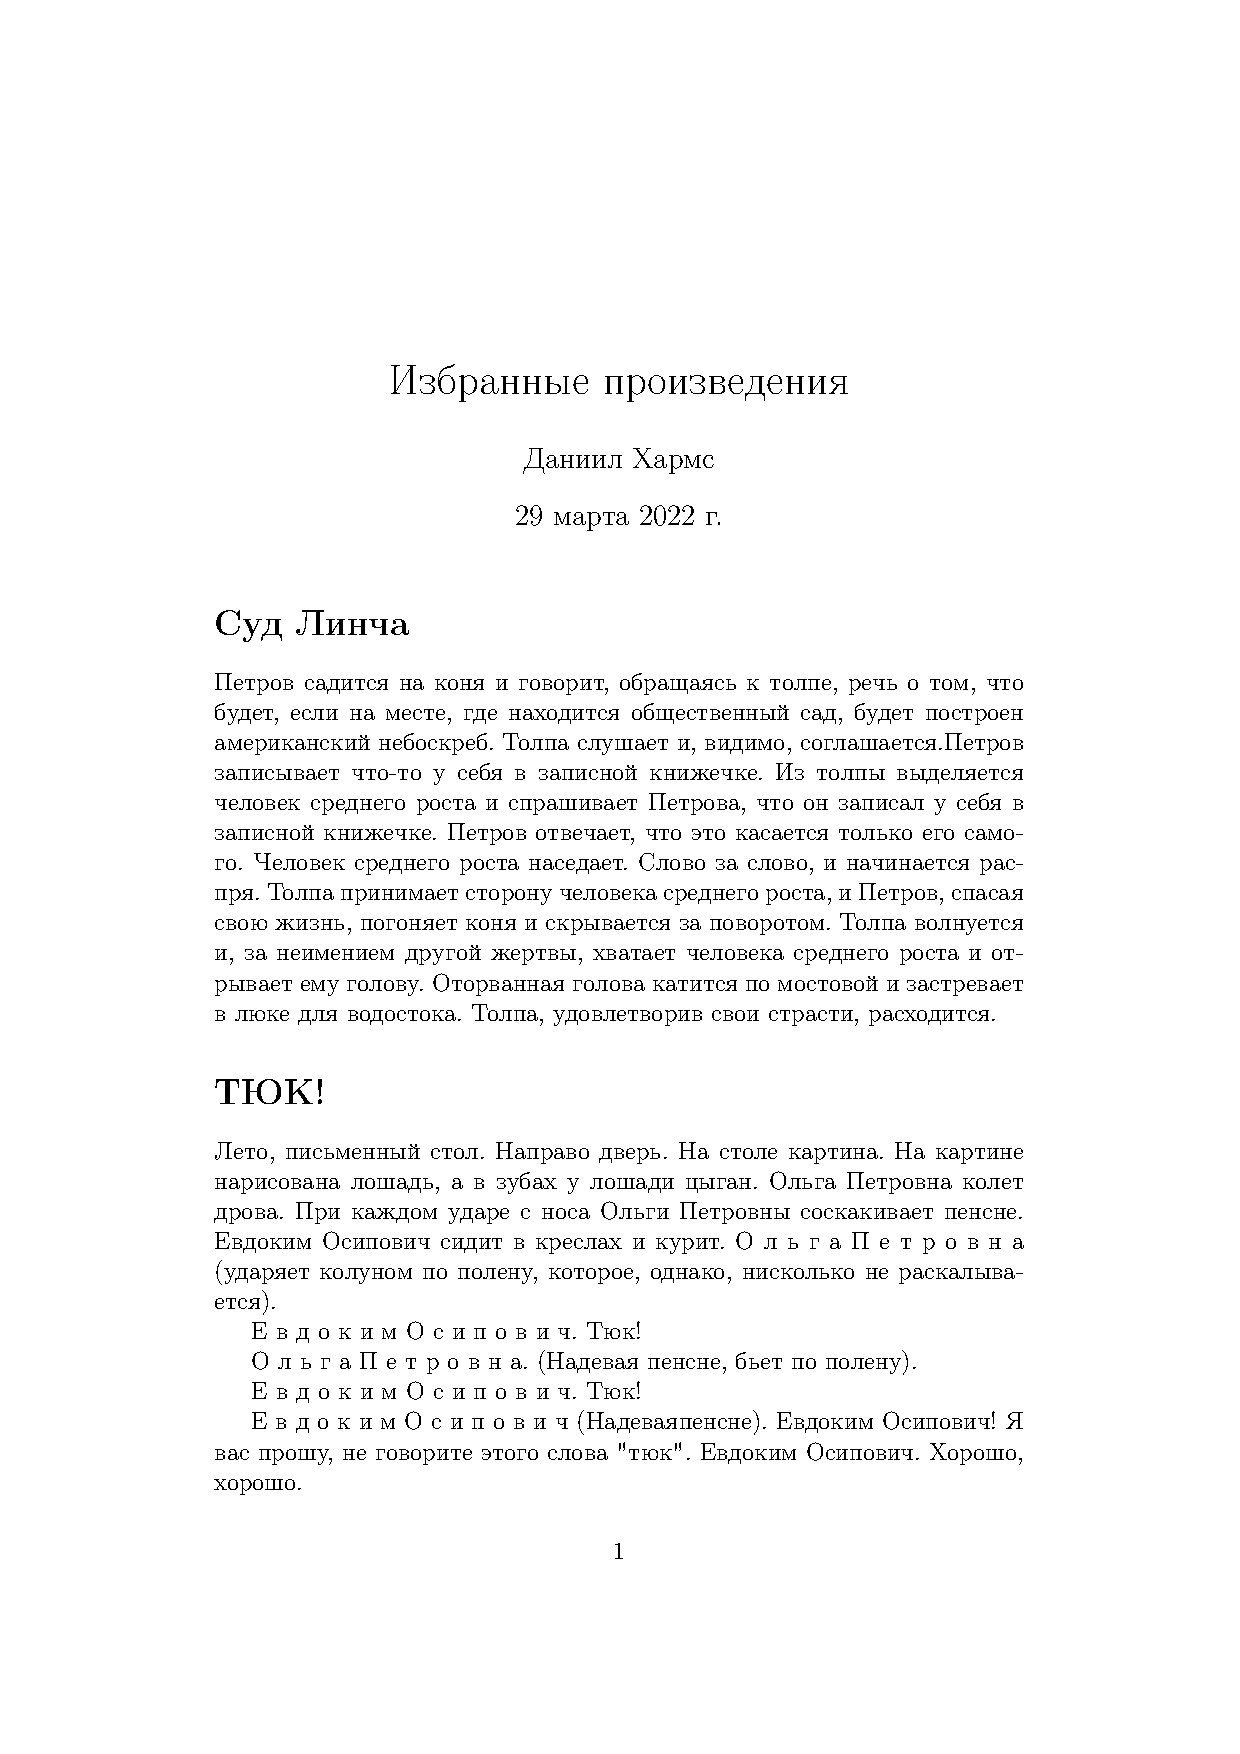
\includegraphics[width = \textwidth]{2.gif}

\caption{Схематическое изображение большого левого вращения}
\end{figure}

Данное вращение используется тогда,
когда (высота $b$"=поддерева; $L$ "--- высота)
$= 2$ и высота $c$"=поддерева $>$ высота $R$.

\subsection*{Малое правое вращение}

%картинка 3
\begin{figure}[ht]
    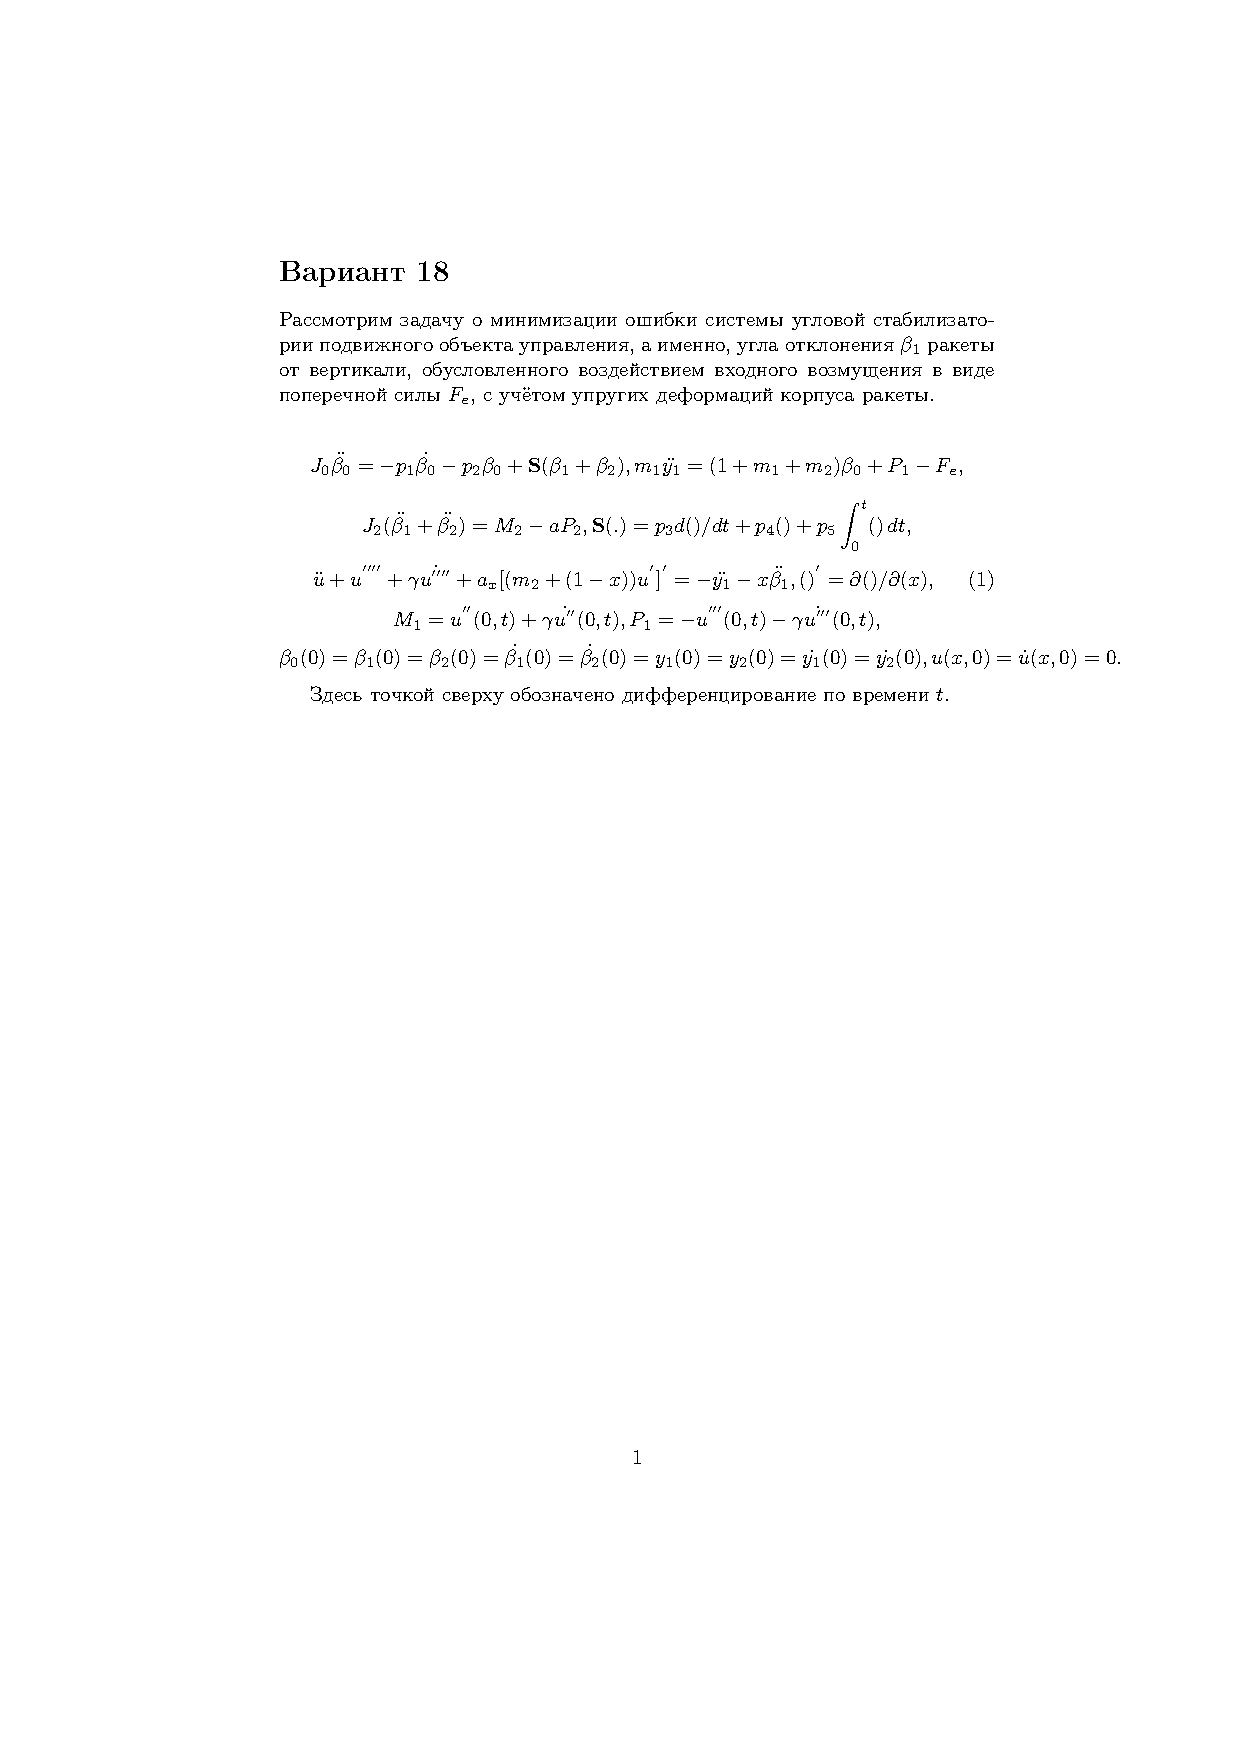
\includegraphics[width = \textwidth]{3.gif}
    
    \caption{Схематическое изображение малого правого вращения}
\end{figure}

Данное вращение используется тогда,
когда (высота $b$"=поддерева "--- высота $R$)
$= 2$ и высота $С \leqslant $ высоты $L$.

\subsection*{Большое правое вращение}

%картинка 4
\begin{figure}[ht]
    \includegraphics[width = \textwidth]{4.gif}
    
    \caption{Схематическое изображение большого правого вращения}

\end{figure}

Данное вращение используется тогда, когда (высота $b$"=поддерева; $R$ "--- высота)
$= 2$ ивысота $c$"=поддерева $ > $ высота $L$.
В каждом случае достаточно просто доказать то, 
что операция приводит к нужному результату и
что полная высота уменьшается не более чем на $1$ и не может увеличиться.
Из-за условия сбалансированности высота дерева $O(\lg(N))$,
где $N$ "--- количество вершин, поэтому добавление элемента требует $Q(\lg(N))$ операций.

    \section*{Алгоритм добавления вершин}
    \input{AlgorithmOfAdd.tex}

    \section*{Алгоритм удаления вершин}
    %\input{AlgorithmOfRemove.tex}

    \section*{Расстановка балансов при удалении}

    \section*{Расстановка при одинарном повороте}

    \section*{расстановка балансов при двойном повороте}

    \section*{Оценка эффективности}

    \section{Список используемой литературы}
\end{document}